\section{Versuchsaufbau und Durchführung}
\subsection{Aufgabe 1: Darstellung des Messsystems}
\subsection{Aufgabe 2: MVC Durchführung}
\subsection{Aufgabe 3: Darstellung der Ergebnisse aus Aufgabe 2}
\subsection{Aufgabe 4: Aufbau des MVC-Versuchsaufbaus}
Wie in Abbildung \ref{fig:measuring_electrodes} und \ref{fig:GND_electrode_c7} zu erkennen ist, besteht der MVC-Versuchsaufbau aus mehreren Komponenten. Es wurden drei Elektroden, vergleichbare zu denen, 
die schon im Lab 2 verwendet wurden, am Probanten angebracht. Eine auf dem Bauch des Bizeps Brachii, eine zwei Zentimeter weiter in Richtung
der Sehne, \ref{fig:measuring_electrodes}, und eine Referenzelektrode auf dem C7 Halswirbel, \ref{fig:GND_electrode_c7}. Die Platzierung der Groundreferenzelektrode auf dem C7-Wirbel wurde gewählt, um
Störungen oder andere Artefakte durch Bewegung zu minimieren.
\begin{figure}[h]
    \centering
    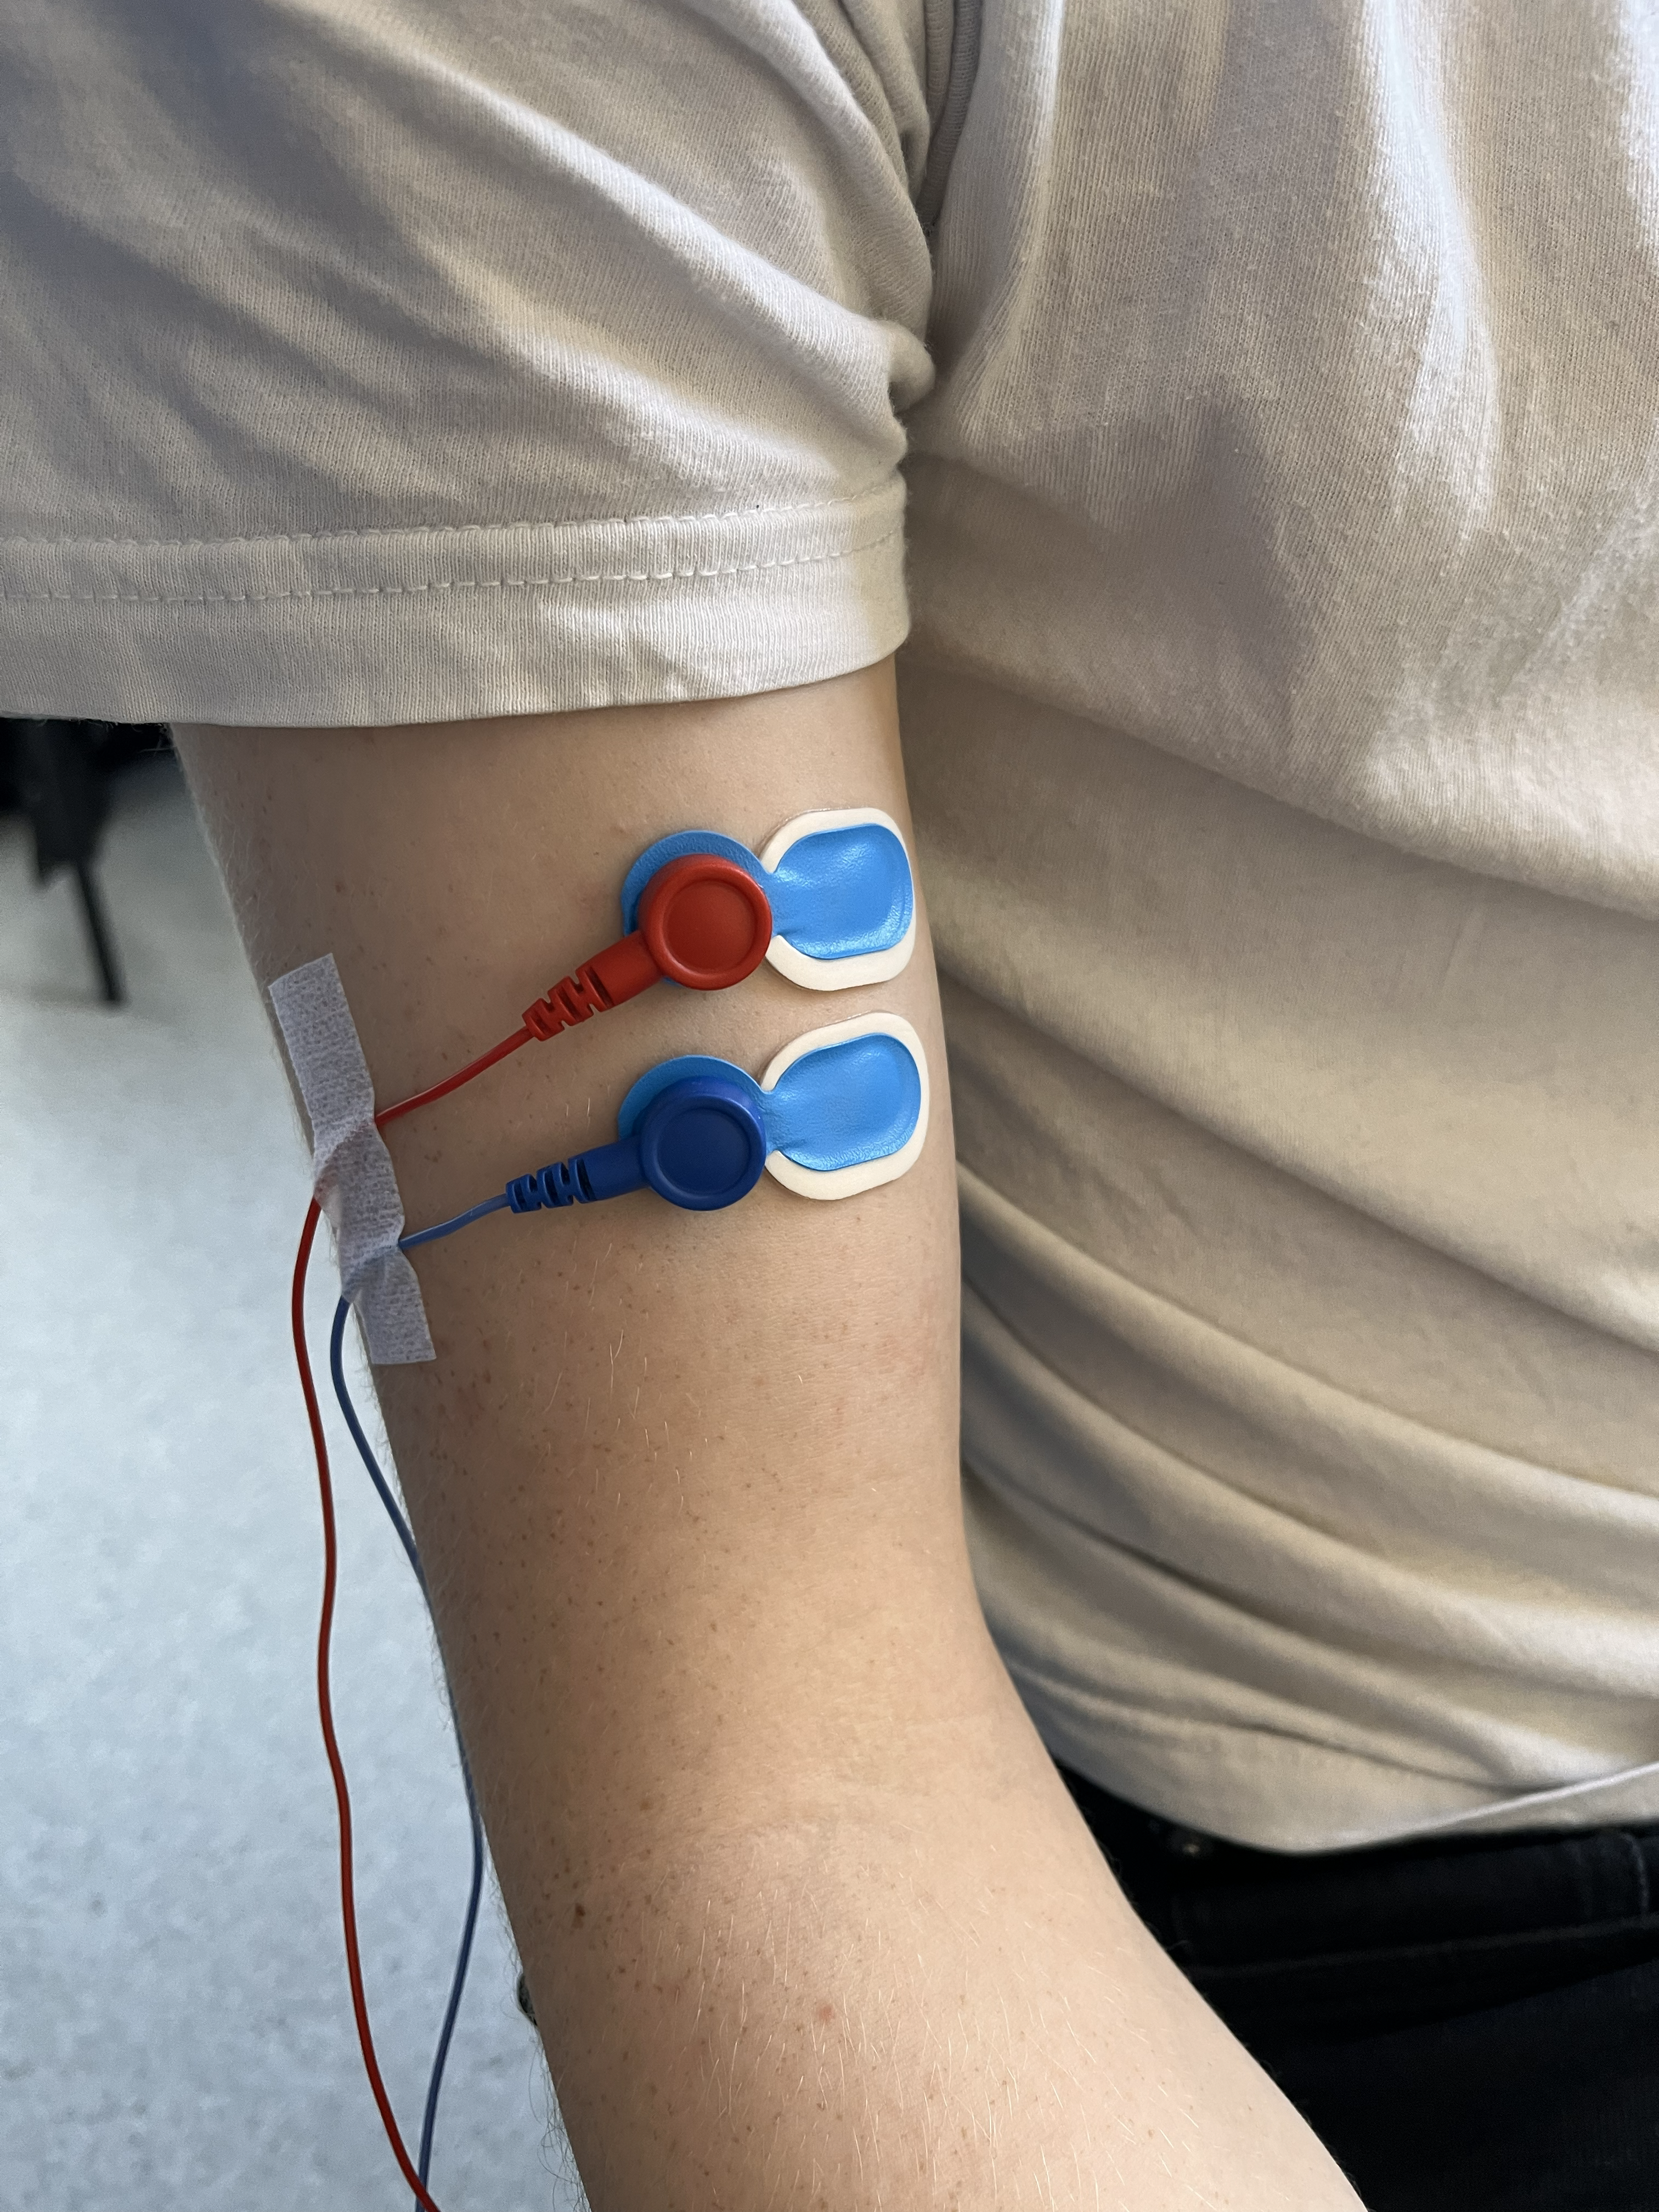
\includegraphics[width=0.3\textwidth]{figures/measuring_electrodes.png}
    \caption{Platzierung der Messelektroden für den MVC-Versuch}
    \label{fig:measuring_electrodes}
\end{figure}
\begin{figure}[h]
    \centering
    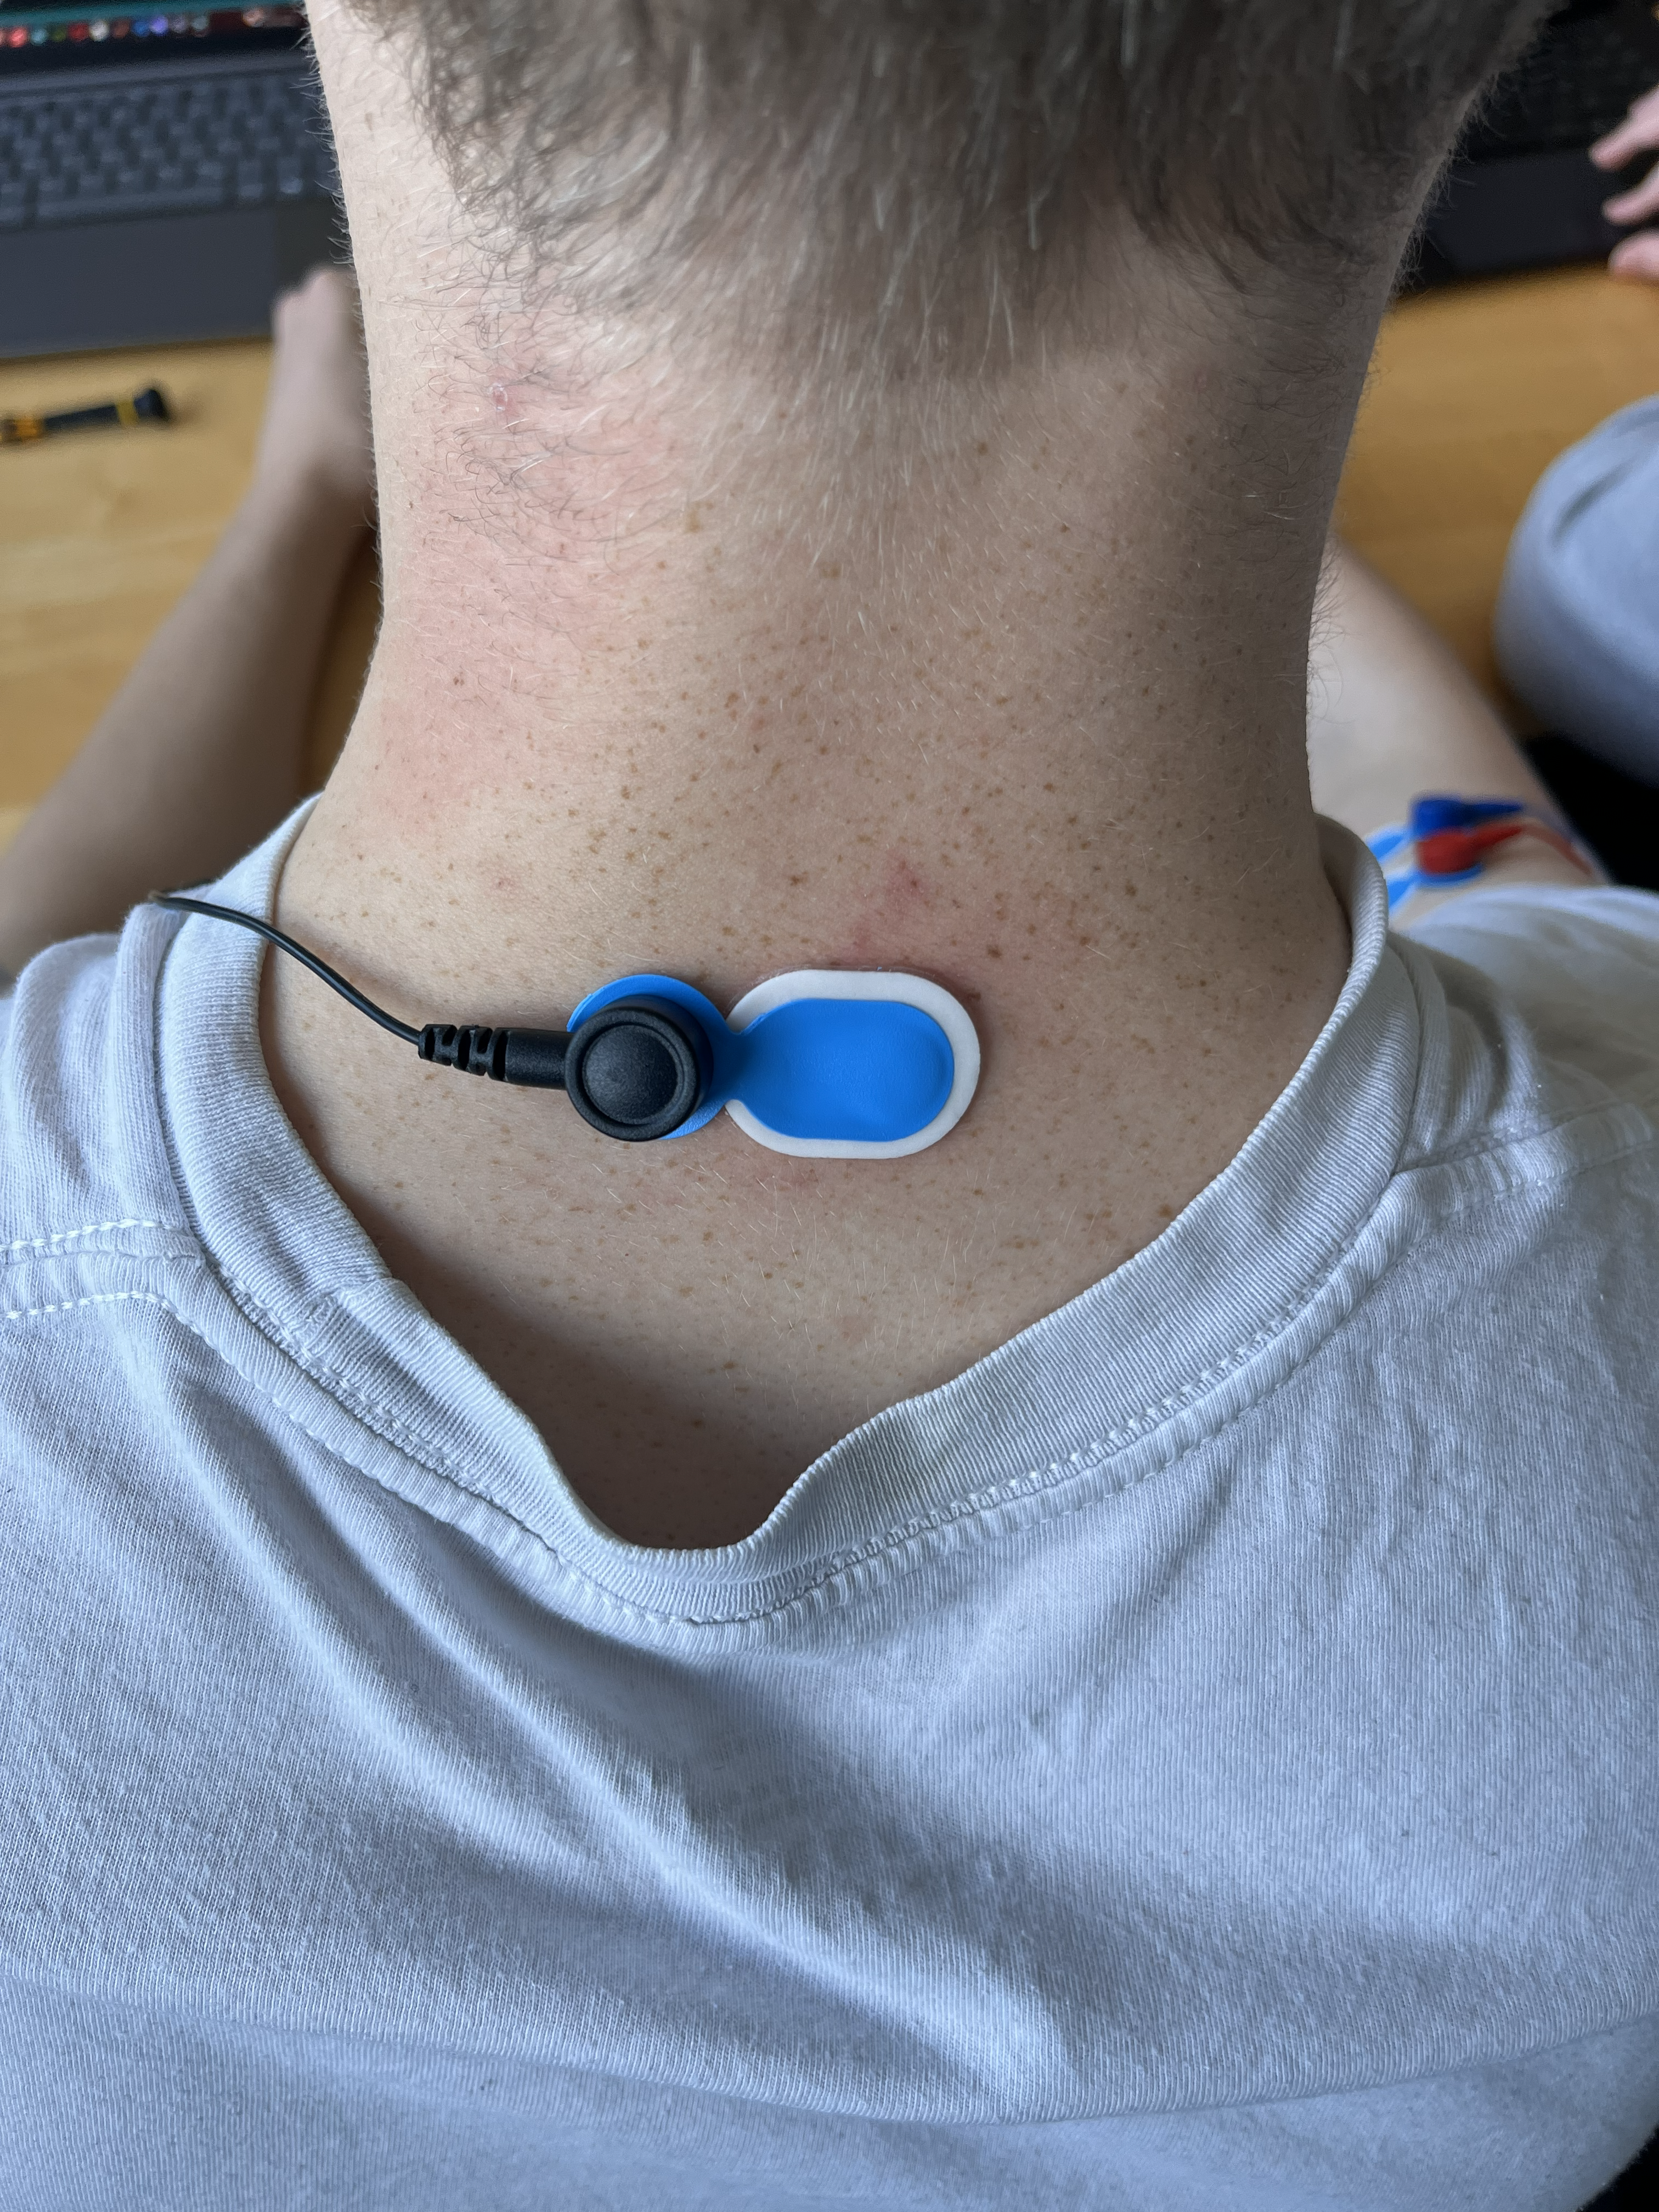
\includegraphics[width=0.3\textwidth]{figures/GND_electrode_c7.png}
    \caption{Platzierung der GND-Elektrode auf dem C7-Wirbel}
    \label{fig:GND_electrode_c7}
\end{figure}
In Abbildung \ref{fig:biceps_tension} ist zu sehen, dass der Probant auf einem Stuhl sitzt, sodass der Unterarm auf dem Oberschenkel aufliegt und sich mit kleinster Bewegung ein 90°-Winkel zwischen
Ober- und Unterarm bildet. Das Handgelenk liegt dann an der Unterkante des Tisches an. Um die MVC zu bestimmen, wird der Probant angewiesen,
so stark wie möglich den Tisch anzuheben, während eine weitere Person auf dem Tisch sitzt, um zu gewährleisten, dass der sich sich nicht
bewegt, obwohl die maximale Kraft vom Probanten aufgebracht wird.
\begin{figure}[h]
    \centering
    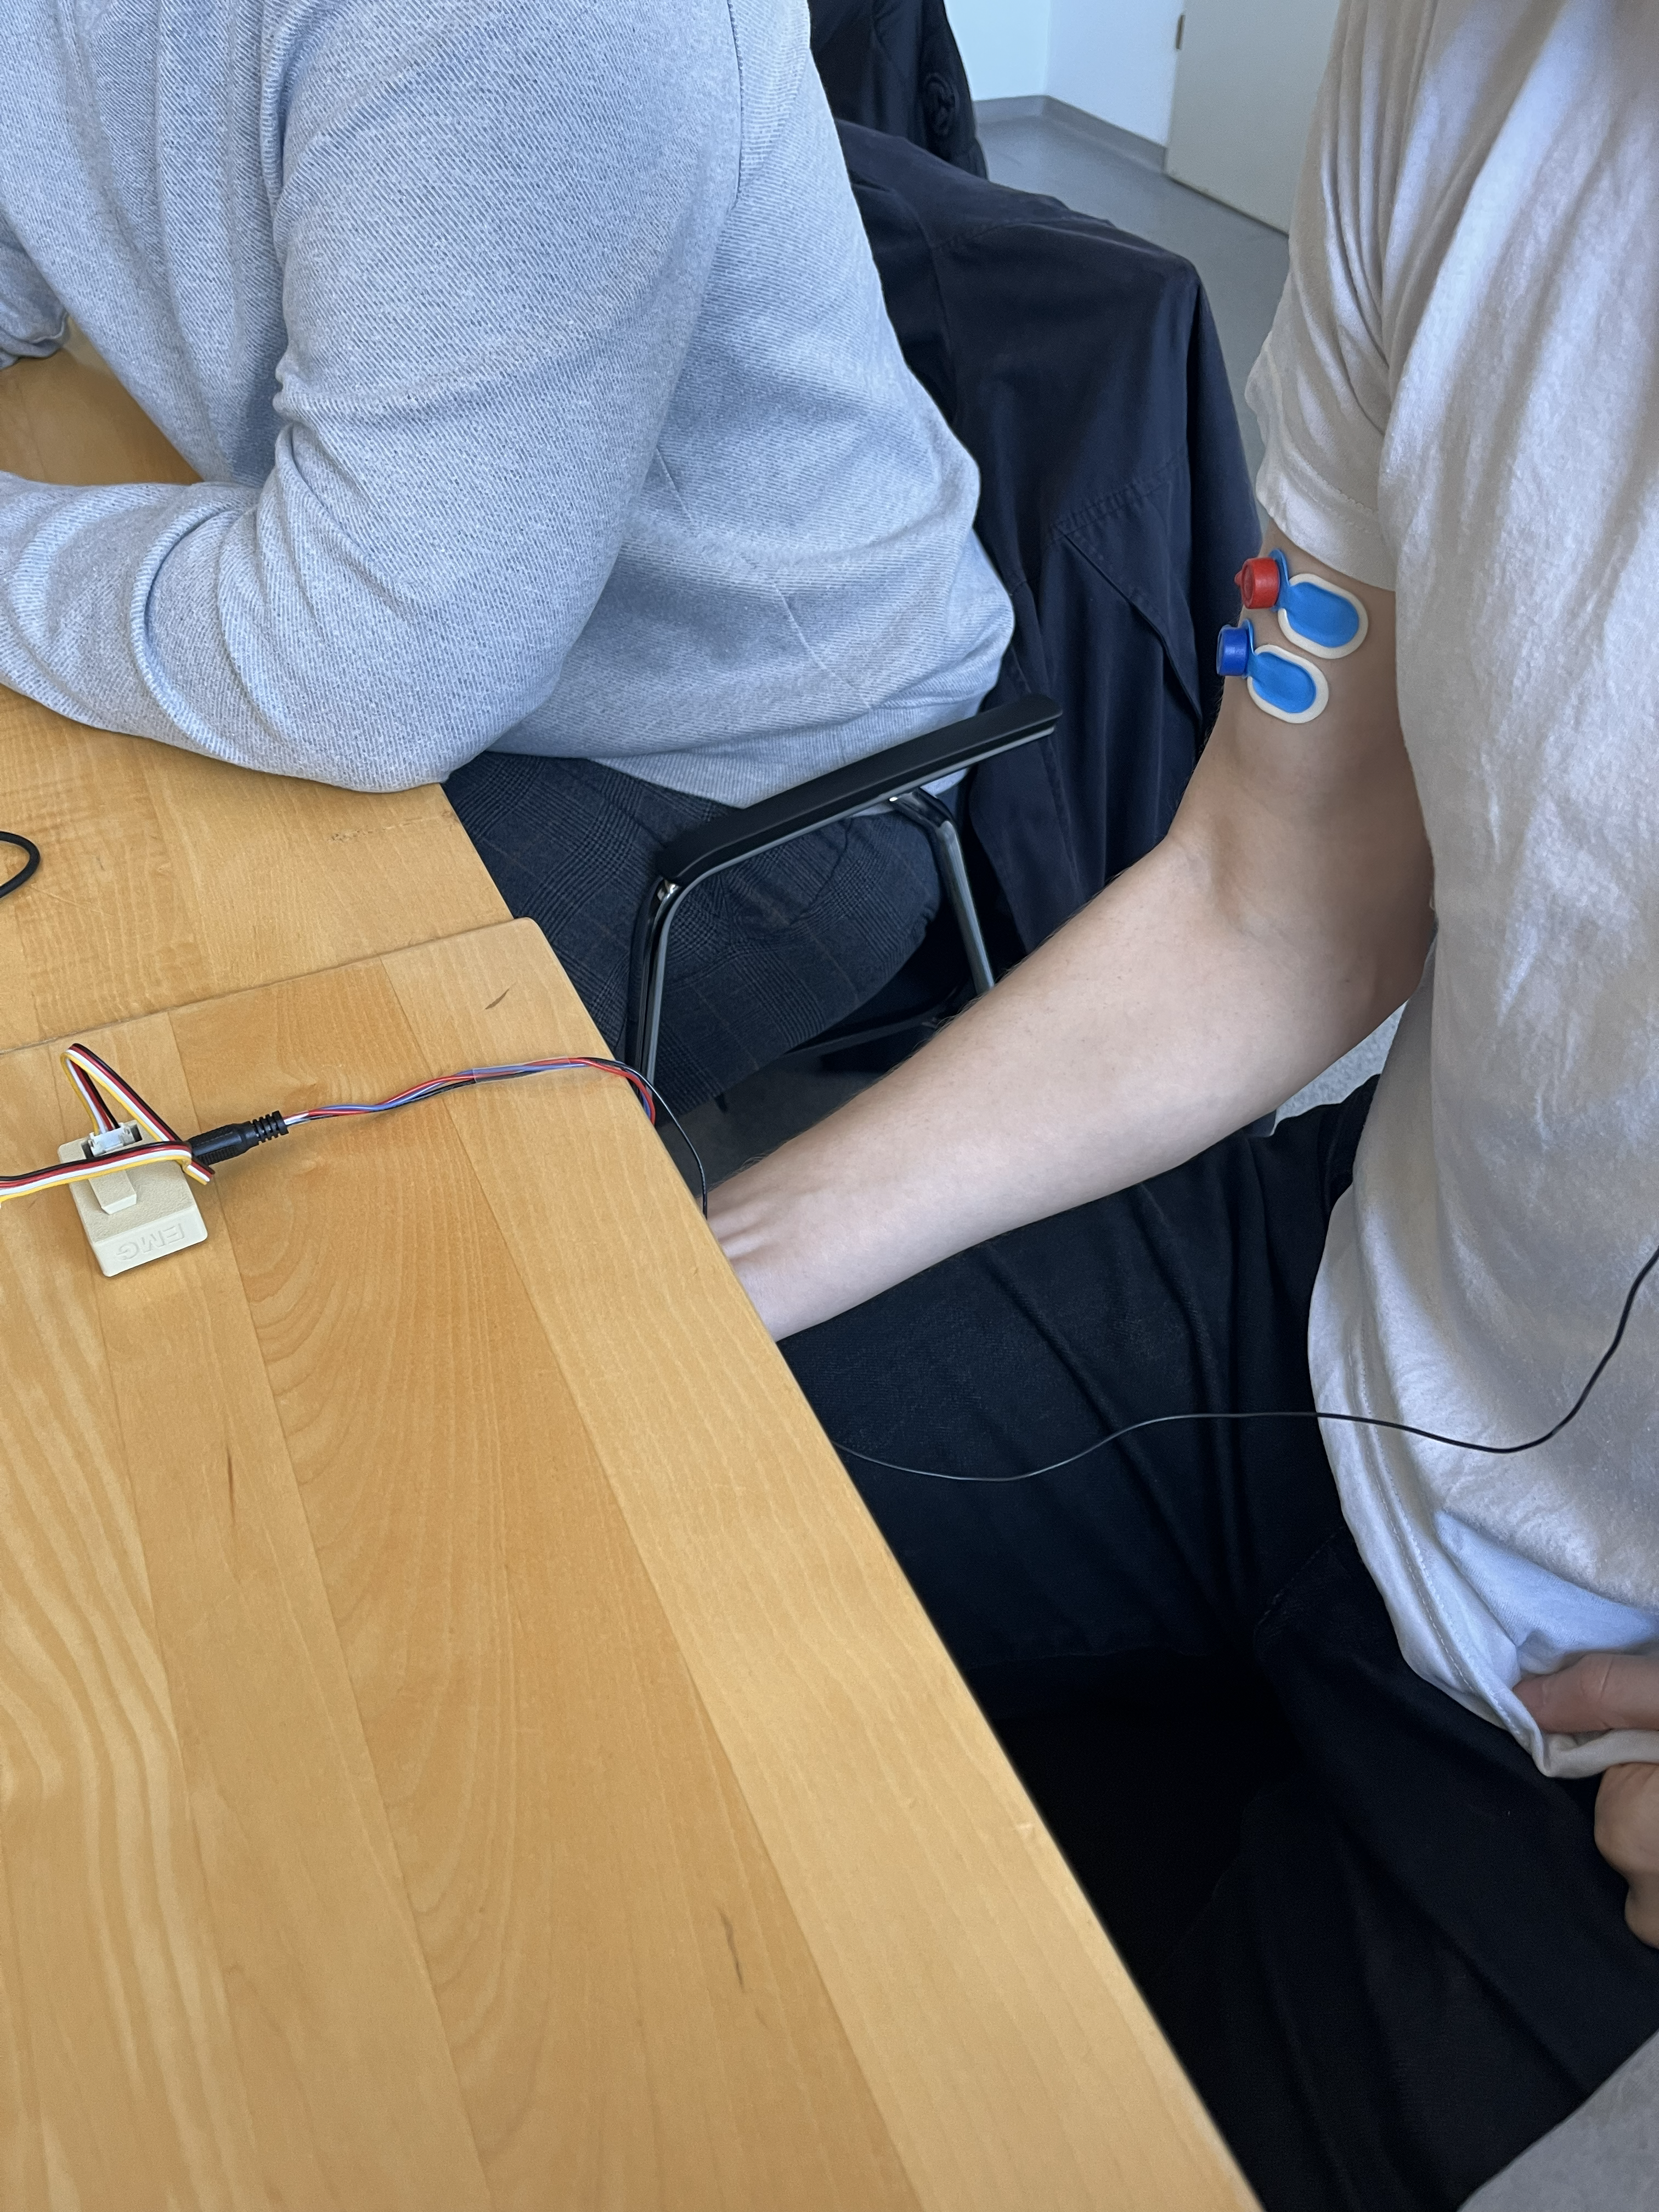
\includegraphics[width=0.4\textwidth]{figures/biceps_tension.png}
    \caption{Angespannter Zustand des Bizeps während des MVC-Versuchs}
    \label{fig:biceps_tension}
\end{figure}
Der Probant hält diese maximale Anspannung für acht bis zehn Sekunden, während die EMG-Daten aufgezeichnet werden. Dieser Vorgang wird
drei Mal wiederholt, mit einer Pause von etwa einer Minute zwischen den Versuchen, um Muskelermüdung zu vermeiden. Der MVC-Versuch wurde für
alle drei Gruppenmitglieder durchgeführt.
\newline
Der Bizeps Brachii lässt sich in diesem Versuchsaufbau maximal kontrahieren, da sich um eine isometrische Kontraktion handelt und dadurch kein Kraftverlust durch Beschleunigung auftritt.
Zudem bedeutet der 90°-Winkel zwischen Ober- und Unterarm, dass der Bizeps in einer optimalen Länge für die maximale Kraftentwicklung ist.
\subsection{Aufgabe 5: Experiment 2 -Relative Muskelaktivierung}
\subsection{Aufgabe 6: Experiment 3 - Ermüdung}
\subsection{Aufgabe 7: Darstellung des Leistungsspektrums}
\subsection{Aufgabe 8: Medianfrequenz des Leistungsspektrums}